% Master Diagram 4 -- 4-bit ripple-carry adder (block diagram)
% Base for Q6 (datapath ALU block), Q7 (one element), Q9 (cascade), Q14 (ALU)
% Loop is unrolled on purpose (avoids \foreach) and uses "\path ... node".
\documentclass[border=10pt]{standalone}
\usepackage{tikz}
\begin{document}
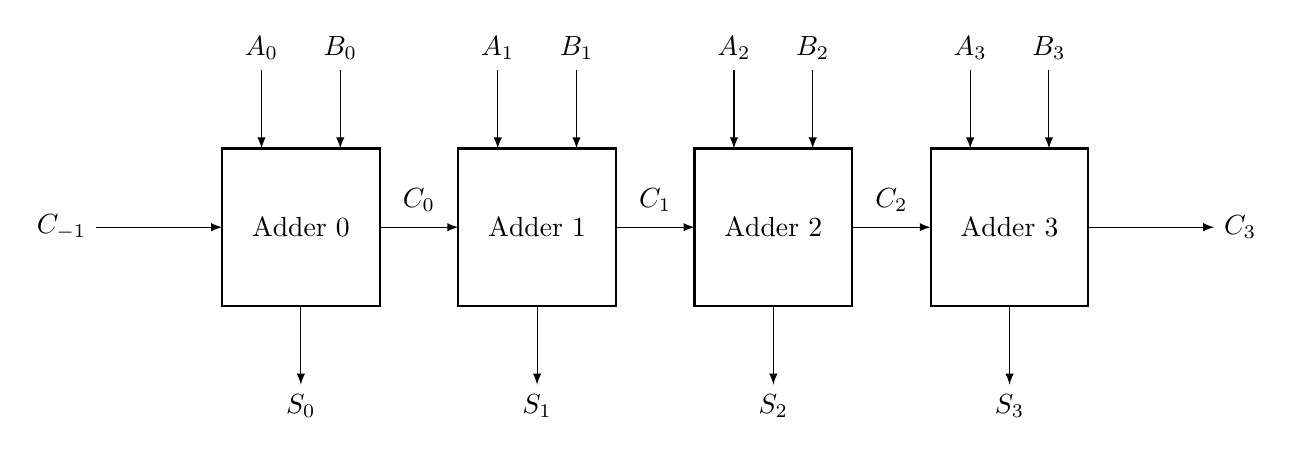
\begin{tikzpicture}[>=latex]
% Adder 0
\draw[thick] (0,0) rectangle (2,2);
\path (1,1) node{Adder 0};
\draw[->] (0.5,3) node[above]{$A_0$} -- (0.5,2);
\draw[->] (1.5,3) node[above]{$B_0$} -- (1.5,2);
\draw[->] (1,0) -- (1,-1) node[below]{$S_0$};
% Adder 1
\draw[thick] (3,0) rectangle (5,2);
\path (4,1) node{Adder 1};
\draw[->] (3.5,3) node[above]{$A_1$} -- (3.5,2);
\draw[->] (4.5,3) node[above]{$B_1$} -- (4.5,2);
\draw[->] (4,0) -- (4,-1) node[below]{$S_1$};
% Adder 2
\draw[thick] (6,0) rectangle (8,2);
\path (7,1) node{Adder 2};
\draw[->] (6.5,3) node[above]{$A_2$} -- (6.5,2);
\draw[->] (7.5,3) node[above]{$B_2$} -- (7.5,2);
\draw[->] (7,0) -- (7,-1) node[below]{$S_2$};
% Adder 3
\draw[thick] (9,0) rectangle (11,2);
\path (10,1) node{Adder 3};
\draw[->] (9.5,3) node[above]{$A_3$} -- (9.5,2);
\draw[->] (10.5,3) node[above]{$B_3$} -- (10.5,2);
\draw[->] (10,0) -- (10,-1) node[below]{$S_3$};
% carry chain (left to right)
\draw[->] (-1.6,1) node[left]{$C_{-1}$} -- (0,1);
\draw[->] (2,1) -- (3,1);  \path (2.5,1.35) node{$C_0$};
\draw[->] (5,1) -- (6,1);  \path (5.5,1.35) node{$C_1$};
\draw[->] (8,1) -- (9,1);  \path (8.5,1.35) node{$C_2$};
\draw[->] (11,1) -- (12.6,1) node[right]{$C_3$};
\end{tikzpicture}
\end{document}
